\chapter{The Effect of Wind Waves on Sediment Permeability}
\label{kap-waves}

ABSTRACT

\section{Introduction}

Permeability is a measure of the resistance to the flow of water 
through the sediment. Cohesive sediments are considered to be non-permeable, 
while sands allow pore water flow and exchange of pore water and bottom water 
by hydrodynamically imposed pressure differences. 
Biogeochemical processes in the sediment are strongly affected by this process 
\citep[][]{huettel2003}, and potentially permeable sediments are present in 
estimately 70$\%$ of the global shelf seas \citep[][]{boudreau2001, 
forster2003}. Furthermore, \cite{forster2003} showed that a large fraction of 
sediments in the western Baltic Sea is permeable.

Permeability is related to grain size distribution and size and geometry of the 
interstices in the sediment, thus empirical relations to calculate $k$ from 
commonly measured sediment properties have been formulated 
\citep[e.g.][]{krumbein1942, carman1937}. These estimates, however, do not 
agree very well with measured permeability values \citep[][]{rusch2001}, 
yielding that grain size distribution is not the only parameter determining 
permeability. \cite{boudreau2001} pointed out, that even the occassional 
resuspension of sediments maintains permeability of the sediment by 
removing finer particles (``winnowing''). Experimentally, \cite{forster2003} 
found that winnowing nearly doubles the permeability, whilst the presence of a 
fluffy layer decreases it. This yields that permeability depends to a great 
extent on the hydrodynamic conditions near the sea bed. 

In the shallow western Baltic Sea, the impact of wave-induced stress on the 
sediment generally dominates over the stress induced by currents 
\citep[][]{Grant1986}. \cite{jonsson2004} used a wave model to calculate the 
wave-induced bottom friction velocity and compared it with the bottom type 
distribution in the Baltic Sea. The good agreement found in that study suggests 
that the wave-induced bottom friction velocity distribution might also be 
correlated with the permeability distribution.

OUTLINE CHAPTERS

\section{Permeability Map}

\cite{forster2003} constructed a map reflecting the permeability in the western 
Baltic Sea using direct measurements of vertical permeability and estimates 
from grain size distribution and porosity. From 37 samples, hydraulic 
conductivity was measured and converted to permeability. From the same samples, 
grain size distribution was determined. One approximation for the permeability 
is the relation of Krumbein and Monk \citep[][]{krumbein1942}
\begin{equation}
 \label{kKM}
 k_{KM} = 7.5 \times 10^{-4} d_{50}^2 e^{-1.31 \sigma},
\end{equation}
where $d_{50}$ is the median diameter and $\sigma$ the standard deviation of 
the grain size distribution. This relation only holds for sufficiently well 
sorted sediments with $\sigma \leq 0.7$. The formula was found to overestimate 
the permeability, thus \eqref{kKM} was divided by a correction factor of 2.6.  
With this new relation, permeability was estimated from two data sets of grain 
size distribution and interpolated. The data are shown in \fig{perm}.
\begin{figure}[ht]
 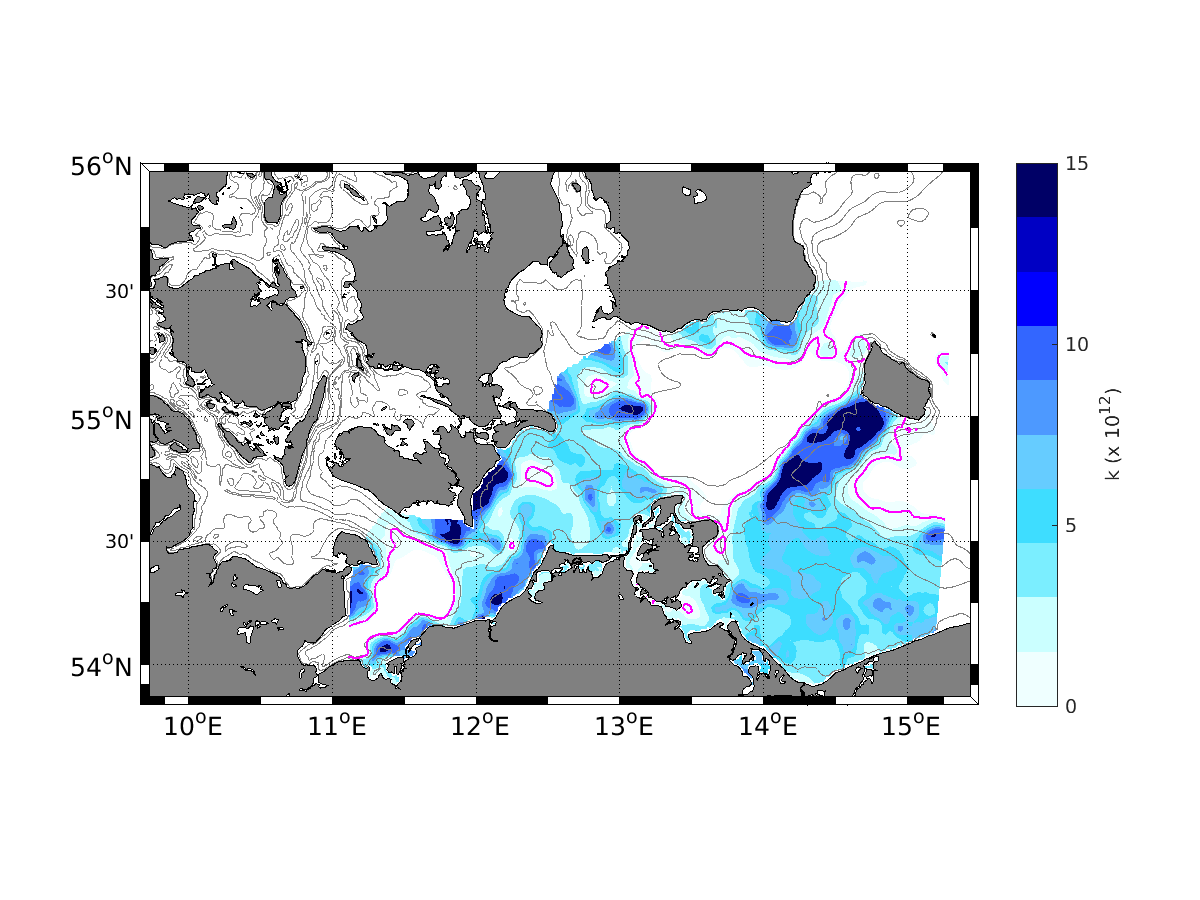
\includegraphics[width=16cm]{bilder/perm_k.png}
 \caption{Permeability data from \cite{forster2003}. Pink line indicates the 
k=$2.5\times10^{-12}$ isoline. Reprinted with permission. \label{perm}}
\end{figure}

\section{Wave model for the Baltic Sea}\label{balticswan}

The SWAN wave model version 41.01 was set up for the Baltic Sea including a 
nesting in the area of the German coastal sea. For the whole Baltic Sea, a grid 
resolution of $0.5^\circ \times 0.1^\circ $ in Latitude and Longitude was chosen 
in a domain reaching from $53.5^\circ \text{N } 9^\circ \text{E}$ to $66^\circ 
\text{N } 31^\circ \text{E}$. This includes the Kattegat, the passage from the 
Baltic to the North Sea, where boundary conditions were prescribed in the east: 
A constant JONSWAP spectrum with a wave height of $1$ m, a period of $5$ s and 
peak wave direction of $90^\circ$ with a high directional spreading. The passage 
from the North to the Baltic sea is very shallow, so the boundary conditions 
have negligible influence on the model outcome. Wave frequency range was set to 
0.1 to 1.8 Hz, which mirrors the actual wave frequencies in the Baltic 
Sea \citep[][]{balticsea}, with a resolution of $42$ frequency bins. 
Computations included a spin-up time of $10$ days, sufficient for wave modeling 
and were performed for the years 2013 and 2014. The model was forced by wind 
data from the German Weather Service (DWD), the computational time step was $1$ 
hour (note that the propagation scheme implemented in SWAN is implicit, so the 
time step is not restricted by numerical issues). 

The nesting area reached from $53.5^\circ \text{N } 10^\circ \text{E}$ to 
$55.5^\circ \text{N } 15^\circ \text{E}$, including the Western German coastal 
seas. Spatial resolution was $0.01^\circ \times 0.025^\circ $ in Latitude and 
Longitude and the computational time step was set to $15$ minutes. Boundary 
conditions came from the Baltic Sea model and all parameters were left 
unchanged.

In \fig{verify} the significant wave height calculated with the wave model was 
compared to data obtained with a wave rider buoy. The significant wave height 
is defined as the average wave height of the highest one-third of the waves. 
This value matches the visually observed wave height best and can be calculated 
from the zeroth-order moment if the variance density spectrum $m_0$ via 
$H_s = 4 \sqrt{m_0}$.
\begin{figure}[ht]
 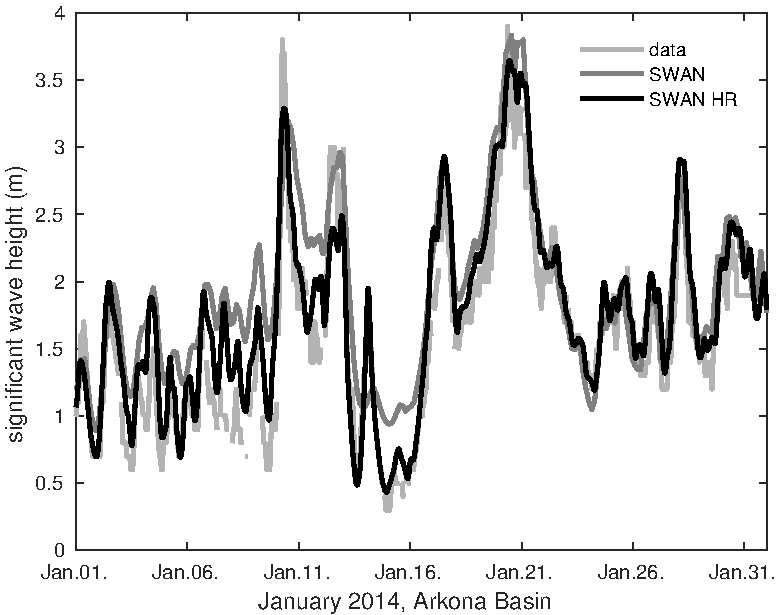
\includegraphics[width=9cm]{bilder/januar.pdf}
 \caption{Significant wave height calculated with the SWAN wave model (HR 
refers to the high resolved nested run) and measured wave height from the 
Arkona wave rider buoy.\label{verify}}
\end{figure}

In the context of a Master Thesis \citep[][]{masterarbeitronja}, the model 
setup for 2013 (still using the previous version SWAN 40.91AB) was 
extensively tested for numerical convergence and compared to measured data on 
several locations in the Baltic Sea. Wave parameters like significant wave 
height were in good agreement with obtained data, even in areas with complex 
topography. A brief description of wind wave properties and processes and a 
discussion the wave model SWAN can be found in Appendix B.

\subsection{Idealized Wind Situations}

Wave-induced resuspension of sediment is related to extreme wind events. Storm 
surges in the Baltic sea are caused by two large-scale wheater 
situations. Strong northwest or northeast winds generate the highest 
waves in the western Baltic \citep[][]{balticsea}. Northeast winds maximize the 
fetch and therefore the wave activity in German coastal waters. Strong 
northwesterly winds occur more frequently, but tend to last shorter. 

To model wave activity under the two scenarios described above, we forced the 
Baltic Sea wave model with constant wind from the northwest (NW) and the 
northeast (NE), respectively. Wind speed was set to 20 m~s$^{-1}$, which was 
the maximal wind speed reached during a strong northwest wind in January 2005.
We used the same resolution and configuration as described in 
section \ref{balticswan} and chose the modeled time period sufficiently long to 
reach stationarity (10 days).

\subsection{Wave-Induced Bottom Friction Velocity}

Bottom friction velocity $u_\ast$ is a common quantity to express the influence 
of waves or currents on the sea bed. It is related to the bottom shear stress 
$\tau_b$ via $u_\ast = \sqrt{\tau_b \slash \rho}$, which on the other hand can 
be estimated as $\tau_b = 0.5 \rho f_w U^2$. Here, $\rho$ is the fluid 
density, $f_w$ the wave friction factor and $U$ the wave-induced
maximal near bottom orbital velocity \citep[][]{schwartz2006}. Hence the 
relation
\begin{equation}
 \label{ustar}
 u_\ast = U \sqrt{0.5 f_w}
\end{equation}
follows. $U$ depends on significant wave height $H_s$, wave length 
$L$, water depth $D$ and wave period and is calculated in the numerical 
model using linear wave theory \citep[][]{holthuijsen2007, schwartz2006}. The 
wave friction factor can either be estimated using median grain size 
\citep[][]{swart1974, nielsen1992} or from the Reynolds number $Re$ 
\citep[][]{nielsen1992, jonsson2004}. As the median grain size is already used 
in the estimation of permeability, we decided to calculate $f_w$ in as a 
function of $Re$ according to
\begin{equation}
 \label{fw}
 f_w = \left\{ \begin{array}{lll}
             \frac{2}{\sqrt{Re}}, & \qquad \qquad \; \,  Re \leq 3 \times 10^5 
\\
              3.34 \times 10^{-3} + 1.05 \times 10^{-9} Re, \, &3 \times 10^5 < 
							  Re < 1 \times 10^6 \\
	      0.024 Re^{-0.123}, \, &1 \times 10^6 \leq Re. \\
              \end{array} 
              \right. 
\end{equation}
The Reynolds number is a quantity to distinguish between laminar and turbulent 
flows, and in this case defined as
\begin{equation}
 \label{reynolds}
 Re = \frac{U H_s}{2 \nu \sinh (2 \pi D \slash L) },
\end{equation}
with $\nu = 1.3 \times 10^{-6}$ m$^2$~s$^{-1}$ being the kinematic viscosity.
\section{Results}	

\subsection{Realistic run}
\begin{figure}[ht]
 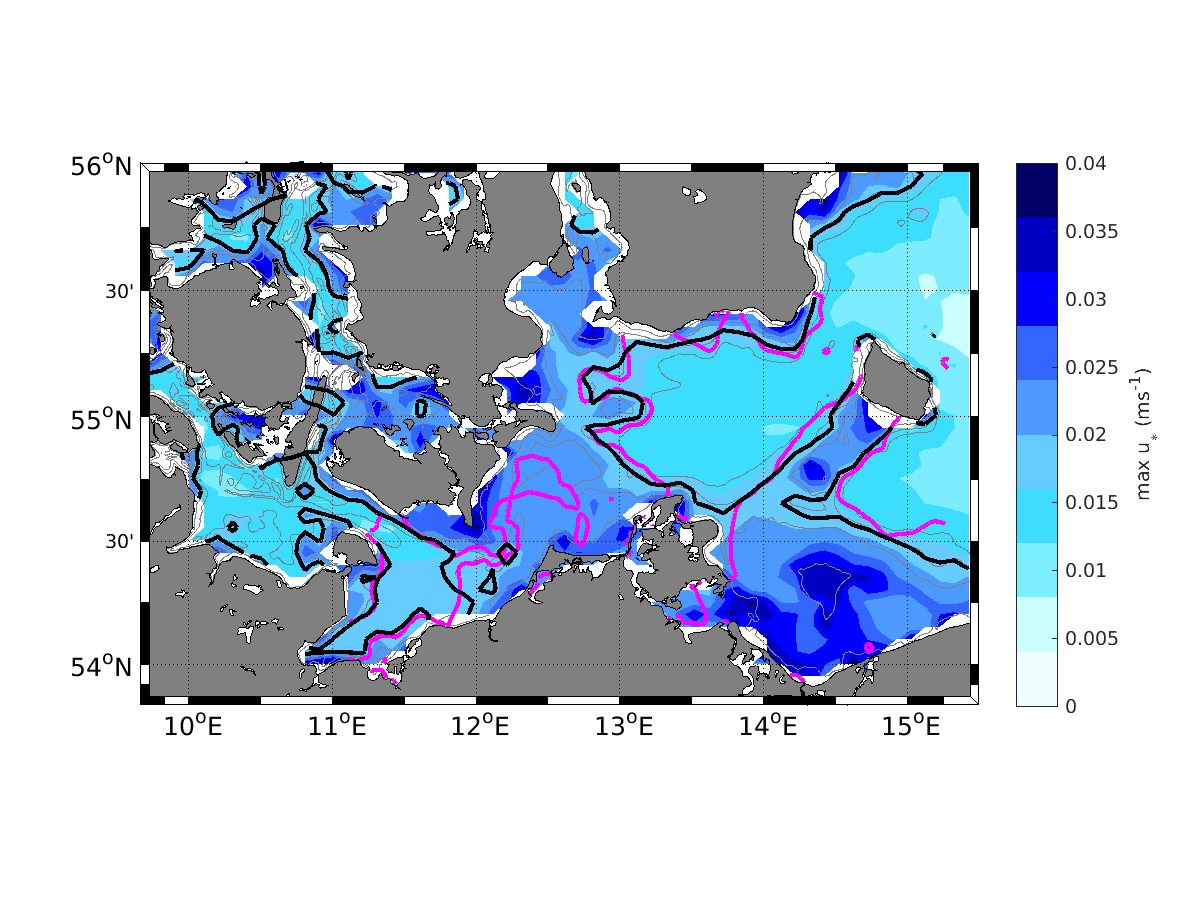
\includegraphics[width=16cm]{bilder/ubot_real.png}
 \caption{Maximal calculated $u_\ast$ using model outcome with realistic 
forcing from the year 2014. Gray lines are isobaths, the pink line is again the 
$k=2.5\times 10^{-12}$ isoline and the black line indicates $u_\ast = 0.02$ 
m~s$^{-1}$.\label{ustar_real}}
\end{figure}

\begin{figure}[ht]
 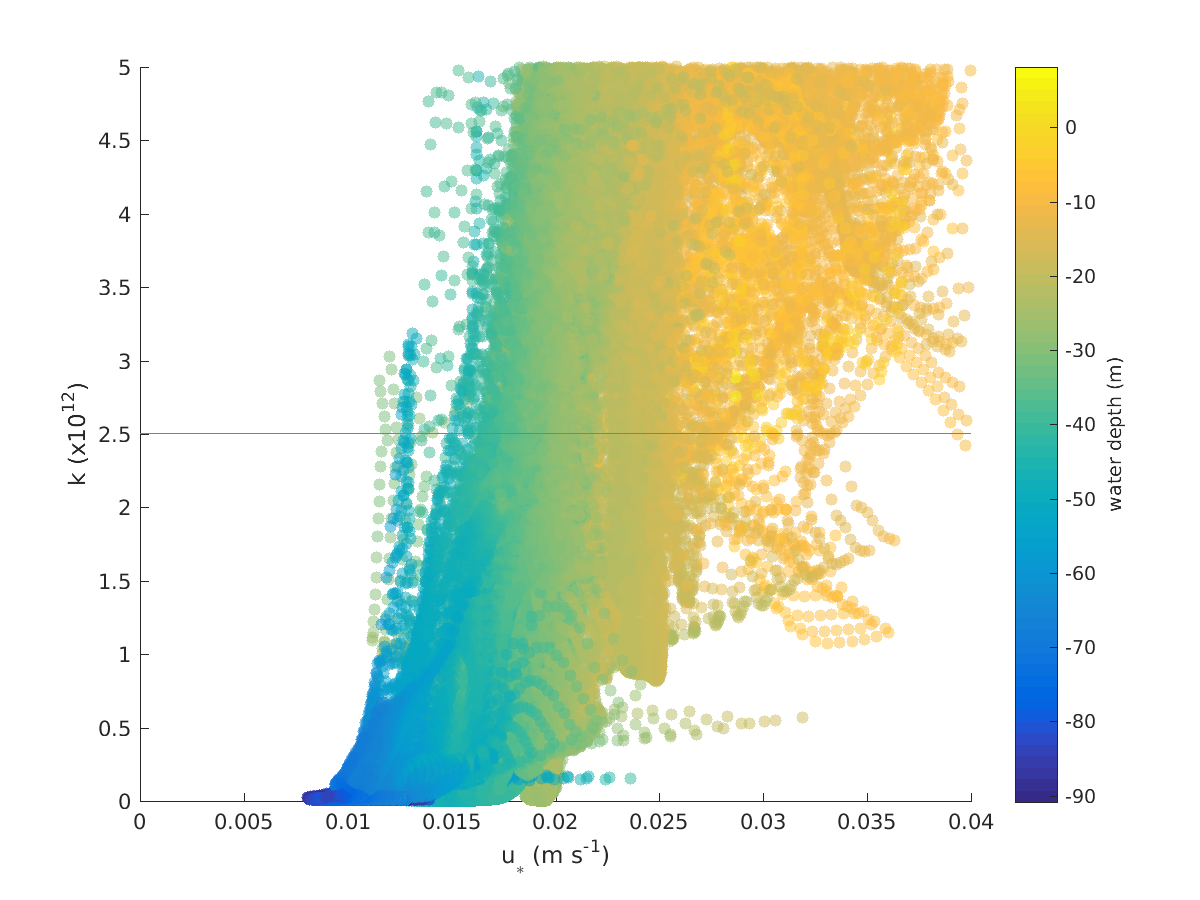
\includegraphics[width=11cm]{bilder/scatter_real.png}
 \caption{Scatter plot of $u_\ast$ and $k$. Colors indicate 
the water depth.\label{scatter_real}}
\end{figure}

\subsection{Idealized cases}

\section{Discussion}

\section{Conclusions}